%%%% ijcai17.tex

\typeout{IJCAI-17 Instructions for Authors}

% These are the instructions for authors for IJCAI-17.
% They are the same as the ones for IJCAI-11 with superficical wording
%   changes only.{\tiny {\tiny {\tiny {\tiny }}}}

\documentclass{article}
% The file ijcai17.sty is the style file for IJCAI-17 (same as ijcai07.sty).
\usepackage{ijcai17}
 \usepackage{amsmath}
 \usepackage{graphicx}
 \usepackage{makecell}
 \usepackage{listings}
 \usepackage{xcolor} 
% Use the postscript times font!
\usepackage{times}

% the following package is optional:
%\usepackage{latexsym} 

% Following comment is from ijcai97-submit.tex:
% The preparation of these files was supported by Schlumberger Palo Alto
% Research, AT\&T Bell Laboratories, and Morgan Kaufmann Publishers.
% Shirley Jowell, of Morgan Kaufmann Publishers, and Peter F.
% Patel-Schneider, of AT\&T Bell Laboratories collaborated on their
% preparation.

% These instructions can be modified and used in other conferences as long
% as credit to the authors and supporting agencies is retained, this notice
% is not changed, and further modification or reuse is not restricted.
% Neither Shirley Jowell nor Peter F. Patel-Schneider can be listed as
% contacts for providing assistance without their prior permission.

% To use for other conferences, change references to files and the
% conference appropriate and use other authors, contacts, publishers, and
% organizations.
% Also change the deadline and address for returning papers and the length and
% page charge instructions.
% Put where the files are available in the appropriate places.

\title{Project 3: Movement Decoding for Brain Computer Interfaces}
\author{Yufeng Yuan\\ 
yy208@duke.edu}

\begin{document}

\maketitle

\begin{abstract}
In this project, a support vector machine should be implemented to classify the communication between brain and computers. All the communications should be classified into two classes, left movement and right movement. Therefore, this is a two-class supervised learning problem which can be solved by SVM.

\end{abstract}

\section{Overview}
In this project, we implemented a SVM classifier to classify the brain signals into two classes.
First, I implemented a SVM classifier for this problem. I used mosekopt() function from MOSEK to solve the quadratic optimization during the training process.
Furthermore, I used 2-level cross-validation to avoid over-fitting. The 1st-level cross-validation segmented the dataset into 6 folds for better test accuracy. The 2nd-level cross-validation uses the five folds in training set to determine the optimal $ \lambda $ for regularization.
Eventually, I added data preprocessing to the date before training and significant improvement gained. Meanwhile,I also implemented a simple neural network for this problem as a comparison with SVM.

\section{Mathematical Formulation}

\subsection{Formulation of the Support Vector Machine}
The decision function for the two-class linear SVM, $X$ is the input data, $W$ is the weight of the classifier and $C$ is a constant.
$$
f(X)=W^TX+C
$$
$$
f(X)=\left\{
\begin{aligned}
\ge 0 && (Class & A) \\
< 0 && (Class & B) \\
\end{aligned}
\right.
$$
The following quadratic optimization problem could be constructed in order to determine $W$ and $C$ with maximum margin. $\xi$ is the error of i-th training sample and $\lambda$ is the hyper-parameter determined by cross-validation.
$$
\min_{W,C,\xi} \sum \xi_i + \lambda \cdot W^TW
$$
$$
S.T. \quad y_i \cdot (W^TX_i+C) \ge 1 - \xi_i
$$
$$
\xi_i \ge 0
$$
$$
(i=1,2,\cdot, \cdot, \cdot, N)
$$
Because the cost function is the sum of two convex functions, which are linear and quadratic. All the constraints are linear. So the problem is a convex optimization problem which can be solved by convex programming.

\subsection{Mapping to MOSEK input form}
The quadratic optimization of SVM formed above can be solve by MOSEK in Matlab. The standard formulation of quadratic optimization in MOSEK is as follows.
$$
minimize \quad  \frac{1}{2}x^TQ^ox+c^Tx+c^f
$$
$$
subject \quad to\quad  l^c_k \le \frac{1}{2}x^TQ^kx+\sum^{n-1}_{j=0}a_{k,j}x_j \le u^c_k, k=0,...,m-1
$$
$$
l^x_j \le x_j \le u^x_j, j=0,...,n-1
$$
According to the formulation of the SVM we derived, we need to minimize the cost function with respect to $W$, $C$, $xi$, so we concatenate these three vectors together and treat it as $x$.
The cost function can be rewritten as 
$$
\frac{1}{2}W^T 2\lambda W + \sum \xi_i
$$
So $Q^k$ and $c^T$ can be derived here
$$
Q^k= 2\lambda, 
c^T = 1
$$
The linear constraint can be rewritten as follows, $a_k^j$ can be derived here
$$
y_i \cdot X_i^T + y_i \cdot C + \xi_i \ge 1
$$
$$
a_{k,j} = [y_j \cdot X_j^T, \quad y_j, \quad 1]
$$
$$
 j=0,...,n-1, k=0,...,m-1
$$
The lower bound of variables is 0, so $l^x_j$ can be derived here
$$
l_j^x = 0, j=0,...,n-1
$$
\subsection{Two-Level Cross Validation}
\subsubsection{1st-Level Six-fold Cross Validation}
The original data set has 120 $\times$ 2 trials, which should be divided into six folds: 20 $\times$ 2 trials per fold. One fold will be used as the test set and the rest will be used as the training set, so the training data has 100 $\times$ 2 trials and teh testing data has 20 $\times$ 2 trials. The accuracy will be tested on all six folds to derive the mean accuracy and standard deviation.
$$
\overline{Ac} = \sum^6_{i=1}Ac(i)/6
$$
$$
stdAc = \sqrt{\frac{1}{6}\sum^6_{i=1}[Ac(i)-\overline{Ac}]^2}
$$
\subsubsection{2nd-Level Five-fold Cross Validation}
Inside the 100$\times$2 trials training data, which should be divided into five folds: 20 $\times$ trials per fold. One fold will be used as the validation set and the rest will be used as the training set, so the training data has 80 $\times$ 2 trials and the testing data has 20 $\times$ 2 trials. We use cross validation here to determine the optimal $\lambda$ of SVM.
$$
\lambda \in \{0.01, 1, 100, 10000\}
$$
\section{Experimental Results}

For the first training fold, the values of $W$ of the 5 most dominant values with largest magnitudes and $C$ are shown as Table 1

\begin{table}[htbp]
	\centering{
	\begin{tabular}{|c|c|c|} \hline
		$W$ & feaSubEImg & feaSubEOvert\\ \hline 
		1   &  0.0346  &  0.0014 \\ \hline
		2   &  0.0330  &  0.0013 \\ \hline
		3   &  0.0303  &  0.0010 \\ \hline
		4   &  0.0289  &  0.0009 \\ \hline
		5   &  0.0231  &  0.0008 \\ \hline
		$C$ &  29.3754  &  1.1258 \\ \hline
	\end{tabular}
	\caption{$W$ and $C$ in the first training fold}
}
\end{table}
\raggedright
For the first training fold, the channel weights of the two data set are shown as Figure 1 and Figure 2

\centering{
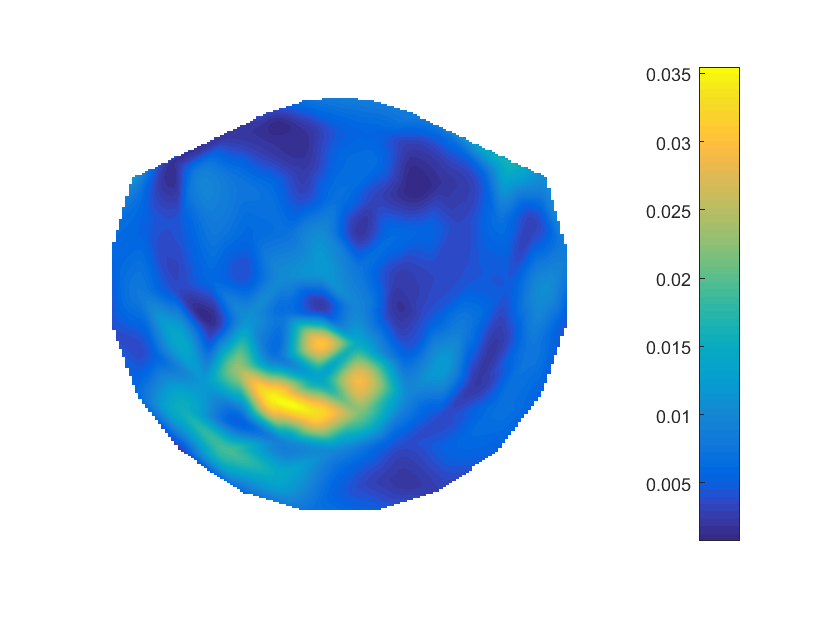
\includegraphics[width=2in,height=2in]{img.png}

Figure 1: The channel weights of feaSubEImg

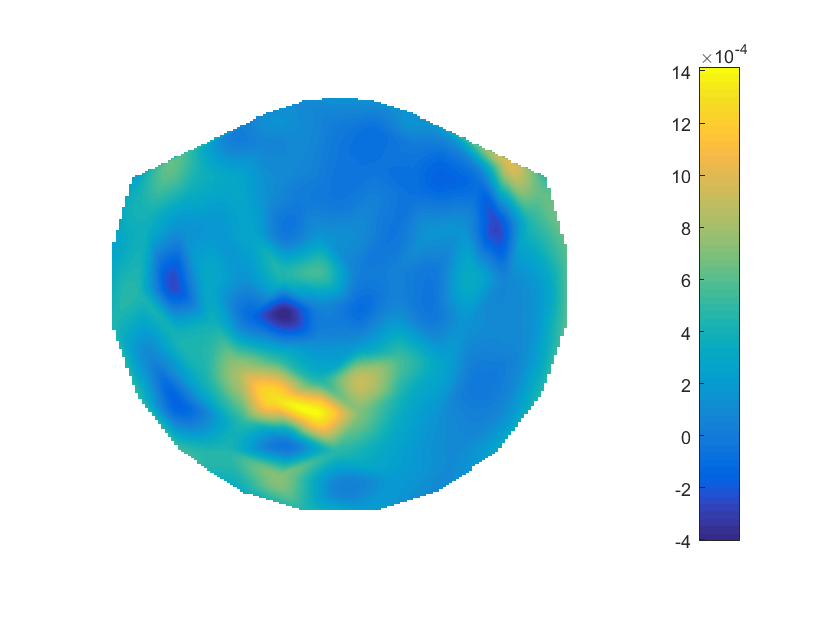
\includegraphics[width=2in,height=2in]{overt.png}

Figure 2: The channel weights of feaSubEOvert

\vspace{1in}
}
\raggedright
The test accuracy of each fold, mean accuracy and standard deviation of all folds are shown as Table 2

\begin{table}[htbp] 
	\centering{
	\begin{tabular}{|c|c|c|} \hline
		  & feaSubEImg & feaSubEOvert\\ \hline 
		Fold 1   &  0.8250  &  0.9000 \\ \hline
		Fold 2   &  0.7750  &  1.0000 \\ \hline
		Fold 3   &  0.8000  &  0.9750 \\ \hline
		Fold 4   &  0.9750  &  1.0000 \\ \hline
		Fold 5   &  0.9000  &  0.9000 \\ \hline
		Fold 6   &  0.9250  &  0.9500 \\ \hline
		Mean     &  0.8667  &  0.9542 \\ \hline
		Std		 &	0.0875  &  0.0459  \\ \hline
	\end{tabular}
	\caption{Fold accuracy, mean accuracy and deviation}
}
\end{table}

The $\lambda$ selected in each fold are shown below as Table 3

\begin{table}[htbp]
	\centering
	\begin{tabular}{|c|c|c|} \hline
		& feaSubEImg & feaSubEOvert\\ \hline 
		Fold 1   &  0.0100  & 100.00  \\ \hline
		Fold 2   &  1.0000  & 100.00  \\ \hline
		Fold 3   &  1.0000  & 100.00  \\ \hline
		Fold 4   &  1.0000  & 0.0100  \\ \hline
		Fold 5   &  0.0100  & 100.00  \\ \hline
		Fold 6   &  100.00  & 10000  \\ \hline
	\end{tabular}
	\caption{Selected $\lambda$ for each fold}
\end{table}\

According to the test accuracy of the two data set, I noticed that the SVM didn't perform very well. One potential reason is that I didn't do data preprocessing. I applied normalization to all the features and significant improvement was observed. The test accuracy, mean accuracy and standard deviation after normalization are shown as Table 4 and Table 5

\begin{table}[htbp]
	\centering
	\begin{tabular}{|c|c|c|} \hline
		& Without & With\\ \hline 
		Fold 1   &  0.9000  &  1.0000 \\ \hline
		Fold 2   &  1.0000  &  1.0000 \\ \hline
		Fold 3   &  0.9750  &  1.0000 \\ \hline
		Fold 4   &  1.0000  &  1.0000 \\ \hline
		Fold 5   &  0.9000  &  1.0000 \\ \hline
		Fold 6   &  0.9500  &  1.0000 \\ \hline
		Mean     &  0.9542  &  1.0000 \\ \hline
		Std		 &	0.0459  &  0.0000  \\ \hline
	\end{tabular}
	\caption{Accuracy of feaSubEOvert with normalization}
\end{table}
\vspace{1in}
\begin{table}[htbp]
	\centering
	\begin{tabular}{|c|c|c|} \hline
		& Without & With\\ \hline 
		Fold 1   &  0.8250  &  1.0000 \\ \hline
		Fold 2   &  0.7750  &  1.0000 \\ \hline
		Fold 3   &  0.8000  &  1.0000 \\ \hline
		Fold 4   &  0.9750  &  0.9750 \\ \hline
		Fold 5   &  0.9000  &  1.0000 \\ \hline
		Fold 6   &  0.9250  &  1.0000 \\ \hline
		Mean     &  0.8667  &  0.9958 \\ \hline
		Std		 &	0.0875  &  0.0102  \\ \hline
	\end{tabular}
	\caption{Accuracy of feaSubEImg with normalization}
\end{table}

Neural network is another powerful algorithm which is capable of doing the task of classification. So I implemented a simple neural network in Python with Keras for this problem. The accuracy it achieved is quite similar to SVM after normalization.

\begin{table}[htbp] 
	\centering{
		\begin{tabular}{|c|c|c|} \hline
			& feaSubEImg & feaSubEOvert\\ \hline 
			Fold 1   &  1.0000  &  1.0000 \\ \hline
			Fold 2   &  1.0000  &  1.0000 \\ \hline
			Fold 3   &  1.0000  &  0.9750 \\ \hline
			Fold 4   &  1.0000  &  0.9750 \\ \hline
			Fold 5   &  1.0000  &  1.0000 \\ \hline
			Fold 6   &  1.0000  &  1.0000 \\ \hline
			Mean     &  1.0000  &  0.9917 \\ \hline
			Std		 &	0.0000  &  0.0129  \\ \hline
		\end{tabular}
		\caption{Fold accuracy, mean accuracy and deviation}
	}
\end{table}


\section{Discussion}
\subsection{Factors that may impact classification accuracy}
\subsubsection{The feature selection of the input data}
The goal of SVM is to find a linear decision boundary between two classes. The more distinct the feature, the easier SVM can classify data into correct categories for better accuracy.
\subsubsection{The selection of $\lambda$}
If the $\lambda$ was large, the cost function would tolerate error while be strict on over-fitting. if the $ \lamdba $ was small, the cost function would tolerate over-fitting while be strict on error. Finding the appropriate $\lambda$ is very important to the accuracy.
\subsubsection{Usaging different kernels}
Here, we are using a very simple linear SVM. It would be hard for it to solve non-linearly-separable cases. Using different kernels instead of linear kernel will make a difference on handling non-separable cases.
\subsection{Limits or problems of this approach}
This problem is a relatively easy problem in classification, so it can be handled by the this approach. However, if the problem becomes complicated, including a lot of non-separable cases, this approach would not be able to obtain current accuracy. Another limit is that if the dimension of the problem becomes much higher than current, the efficiency of this approach will be problematic.
\subsection{Possible improvements that can be done}
We only consider $\lambda$ from [0.01, 1, 100, 10000] to determine the optimal $\lamdba$. If we can set a smaller step size the generate more selection of $\lambda$, we should get more accurate selection of $\lambda$.
More data preprocessing could be done. Instead of using simple normalization, we can use other advanced techniques such as PCA (principle component analysis) or whitening to reduce the dimension of input data.
We can also oollect more data. With more input data, the classifier can be trained on more cases to avoid over-fitting and reduce the standard deviation.
\end{document}

